\documentclass{jsarticle}
\usepackage[dvipdfmx]{graphicx}
\usepackage{amsmath,amssymb}
\usepackage{here}
\usepackage{listings,jlisting}
\usepackage{multirow}
\usepackage{url}
\usepackage{lscape}
\usepackage{bm}
\usepackage[top=10truemm,bottom=15truemm,left=25truemm,right=25truemm]{geometry}
\usepackage{ascmac}
\usepackage{braket}
\usepackage{physics}
\usepackage[dvipdfmx]{color}
\usepackage[dvipdfmx]{hyperref}
\newcommand{\mex}[2]{#1 \times 10^{#2}}
\newcommand{\iex}[2]{$#1 \times 10^{#2}$}
\newcommand{\mr}[1]{\mathrm{#1}}
\newcommand{\arbvt}[2]{#1_{\mbox{\tiny #2}}}
\newcommand{\arbv}[2]{#1_{\mbox{\scriptsize #2}}}
\newcommand{\unit}[2]{#1\,[\mathrm{#2}]}
\newcommand{\un}[1]{\,[\mathrm{#1}]}

\newcommand{\argmax}{\mathop{\rm arg~max}\limits}
\newcommand{\argmin}{\mathop{\rm arg~min}\limits}

%\renewcommand{\lstlistingname}{コード}
%\renewcommand{\thelstnumber}{\tt{\arabic{lstnumber}}}

%\renewcommand{\sfdefault}{phv}
%\renewcommand{\kanjifamilydefault}{\gtdefault}%和文用

%%%%%%%%%%%%%%%%
\lstset{
	%プログラム言語(複数の言語に対応,C,C++も可)
 	language = Python,
 	%背景色と透過度
 	backgroundcolor={\color[gray]{.90}},
 	%枠外に行った時の自動改行
 	breaklines = true,
 	%自動開業後のインデント量(デフォルトでは20[pt])	
 	breakindent = 10pt,
 	%標準の書体
 	basicstyle = \ttfamily\scriptsize,
 	%basicstyle = {\small}
 	%コメントの書体
 	commentstyle = {\itshape \color[cmyk]{1,0.4,1,0}},
 	%関数名等の色の設定
 	classoffset = 0,
 	%キーワード(int, ifなど)の書体
 	keywordstyle = {\bfseries \color[cmyk]{0,1,0,0}},
 	%""で囲まれたなどの"文字"の書体
 	stringstyle = {\ttfamily \color[rgb]{0,0,1}},
 	%枠 "t"は上に線を記載, "T"は上に二重線を記載
	%他オプション:leftline,topline,bottomline,lines,single,shadowbox
 	frame = TBrl,
 	%frameまでの間隔(行番号とプログラムの間)
 	framesep = 5pt,
 	%行番号の位置
 	numbers = none,
	%行番号の間隔
 	stepnumber = 1,
	%右マージン
 	%xrightmargin=0zw,
 	%左マージン
	%xleftmargin=3zw,
	%行番号の書体
 	numberstyle = \tiny,
	%タブの大きさ
 	tabsize = 4,
 	%キャプションの場所("tb"ならば上下両方に記載)
 	captionpos = t
}
%%%%%%%%%%%%%%%%
\renewcommand\floatpagefraction{.001}
\makeatletter
\setlength\@fpsep{\textheight}
\newcommand*{\centerfloat}{%
  \parindent \z@
  \leftskip \z@ \@plus 1fil \@minus \textwidth
  \rightskip\leftskip
  \parfillskip \z@skip}
\makeatother


\makeatletter
\renewenvironment{description}{%
\list{}{%
\labelwidth=\leftmargin
\labelsep=1zw
\advance \labelwidth by -\labelsep
\let \makelabel=\descriptionlabel}}{\endlist}
\renewcommand*\descriptionlabel[1]{\normalfont #1 \hfil}
\makeatother
%%%%%%%%%%%%%%%
\begin{document}
\title{量子情報物理レポート}
\author{37-216657 何 若凡}
\date{2022年1月15日}
\maketitle


\begin{itembox}[l]{問題}
	\vspace*{-0mm}
	\centering
	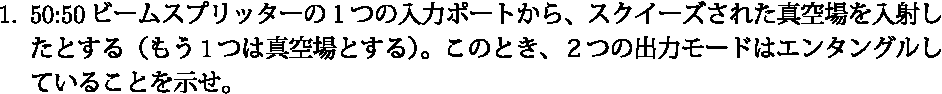
\includegraphics[width=1\linewidth]{./graphics/1.pdf}

方針:エンタングルしている様子をシュレディンガー描像的に見れるようにする。(フォック基底で)
\end{itembox}


まずスクイージング演算子の定義のみ行っておく。\\
$r$は言わずもがな、スクイージングパラメーターである。
\begin{gather*}
	S(r) = e^{\frac{r}{2}(\hat{a}^2 - \hat{a}^{\dagger 2})}\\
	S(r) \hat{a} S^{\dagger}(r) = \hat{a} \cosh r + \hat{a}^{\dagger} \sinh r
\end{gather*}
スクイーズド真空場$\ket{\mathrm{sq}}$を明示的に書き下す。\\
ヌリファイヤーは$S(r)\hat{a}S^{\dagger}(r)$なので、次の方程式を解けばいい。
\begin{gather*}
	(\hat{a} \cosh r + \hat{a}^{\dagger} \sinh r) \ket{\mathrm{sq}} = 0\\
	\ket{\mathrm{sq}} = \sum^{\infty}_{n=0} c_n \ket{n}
\end{gather*}
昇降演算子はフォック基底間で次のように作用する。$\hat{a}\ket{n} = \sqrt{n}\ket{n-1}$、$\hat{a}^\dagger \ket{n} = \sqrt{n+1}\ket{n+1}$。\\
それによって、方程式が次のように変形できるから、それぞれの係数$c_n$に関する連立方程式が作れる。
\begin{gather*}
	\cosh r \sum^{\infty}_{n=0} c_n \sqrt{n} \ket{n-1} + \sinh r \sum^{\infty}_{n=0} c_n \sqrt{n+1} \ket{n+1} = 0
\end{gather*}
係数の方程式は次のようになり、偶数の光子数状態の重ね合わせであることがわかる。
\begin{align*}
	(1)	& c_{n+2} = - \tanh r \sqrt{\frac{n+1}{n+2}} c_n\\
		& \Rightarrow c_{2n} = (-\tanh r)^{n} \sqrt{\frac{(2n-1)!!}{(2n)!!}} c_0 \\
	(2)	& c_1 = 0 \\
		& \Rightarrow c_{\text{奇数}} = 0
\end{align*}
規格化条件を考えれば$c_0 = 1/\sqrt{\cosh r}$となる。計算は次の通り。
\begin{gather*}
	\sum^{\infty}_{n=0} \qty|c_{2n}|^2 = |c_0|^2 \sum^{\infty}_{n=0} \frac{(2n-1)!!}{(2n)!!} (\tanh^2 r)^n = |c_0|^2 \sum^{\infty}_{n=0} \frac{(2n-1)!!}{2^n n!} (\tanh^2 r)^n\\
	\text{マクローリン展開} \qquad \frac{1}{\sqrt{1-x}} = \sum^{\infty}_{n=0} \frac{(2n-1)!!}{2^n n!} x^n \qquad (x = \tanh^2 r \text{を代入})\\
	\sum^{\infty}_{n=0} \qty|c_{2n}|^2 = |c_0|^2 \frac{1}{\sqrt{1-\tanh^2 r}} = |c_0|^2 \cosh r = 1
\end{gather*}
よってスクイーズド真空場は次のように表される。よく見る形である。
\begin{gather*}
	\ket{sq} = \frac{1}{\sqrt{\cosh r}} \qty( \ket{0} - \frac{\tanh r}{\sqrt{2}} \ket{2} + \frac{\sqrt{6} (\tanh r)^2}{4} \ket{4} - \cdots )
\end{gather*}
最初の問題設定に沿って、2モードの真空場を考えてから片方だけにスクイージングを適用する。\\
少し飛躍して恐縮だが、任意の光子数状態を生成演算子によって作る表記にする。
\begin{gather*}
	\ket{\mathrm{sq}, 0} =  \frac{1}{\sqrt{\cosh r}} \sum^{\infty}_{n=0} (- \tanh r)^n \frac{(\hat{a}^{\dagger}_{1})^{2n}}{(2n)!!} \ket{0,0}
\end{gather*}
ようやく、ビームスプリッターを適用できる状態になった。\\
$\hat{B}$をビームスプリッター演算子として、$\hat{B} \ket{\mathrm{sq}, 0}$を求めたい。
50:50のビームスプリッターを考えており、簡単のため適当な位相因子を採用することで$\hat{B} \hat{a}^\dagger_1 \hat{B} = (\hat{a}^\dagger_1 + \hat{a}^\dagger_2)/\sqrt{2}$となるものとする。\\
なお、最後の$\hat{B}^\dagger$は$\ket{0,0} = \hat{B} \ket{0,0}$を根拠に追加している。
\begin{align*}
	\hat{B} \ket{\mathrm{sq}, 0} 	&= \frac{1}{\sqrt{\cosh r}} \sum^{\infty}_{n=0} (- \tanh r)^n \hat{B} \frac{(\hat{a}^{\dagger}_{1})^{2n}}{(2n)!!} \ket{0,0}\\
									&= \frac{1}{\sqrt{\cosh r}} \sum^{\infty}_{n=0} (- \tanh r)^n  \frac{( \hat{B} \hat{a}^{\dagger}_{1} \hat{B}^\dagger )^{2n}}{(2n)!!} \ket{0,0}\\
									&= \frac{1}{\sqrt{\cosh r}} \sum^{\infty}_{n=0} (- \tanh r)^n  \frac{(  \hat{a}^\dagger_1 + \hat{a}^\dagger_2  )^{2n}}{2^n (2n)!!} \ket{0,0}
\end{align*}
ここまでくるとモード1,2がどのようなエンタングルメントを持っているか、わかりそうな気がする。\\
具体的に言語化すると、モード1,2の光子数分布が正の相関を持っているということである。\\
それを明らかにするために、生成演算子をすべて適用してみる。
\begin{align*}
	\hat{B} \ket{\mathrm{sq}, 0} 	&= \frac{1}{\sqrt{\cosh r}} \sum^{\infty}_{n=0} (- \tanh r)^n \frac{1}{2^n (2n)!!} \sum^{2n}_{k=0} {}_{2n} \mathrm{C}_k (\hat{a}^\dagger_1)^k (\hat{a}^\dagger_2)^{2n-k}  \ket{0,0}\\
									&= \frac{1}{\sqrt{\cosh r}} \sum^{\infty}_{n=0} (- \tanh r)^n \frac{1}{2^n (2n)!!} \sum^{2n}_{k=0} {}_{2n} \frac{(2n)!}{\sqrt{k!} \sqrt{(2n-k)!}} \ket{k,2n-k}
\end{align*}
上の式は光子数が$k$やら$2n-k$やらでわかりにくいため、適当に置き換えるとよい。\\
平たく言えばモード1,2の光子数が$n_1,n_2$になる確率は次のようになる。
\begin{gather*}
	P(n_1,n_2) = \frac{(-\tanh r)^{n_1 + n_2}}{\cosh r} \frac{1}{2^{n_1 + n_2}} \frac{1}{n_1 ! n_2 !} \frac{(n_1+n_2)!^2}{(n_1+n_2)!!^2} 
	\qquad (n_1+n_2\text{が偶数の時のみ。他は0})
\end{gather*}
光子数分布の確率式からエンタングルメントの存在を認めることは難しいが、\\
グラフにプロットすると明らかにエンタングルしていることがわかる。\\
下のグラフはスクイージングが$r=10$の時のBSモード1,2の光子数分布である。\\


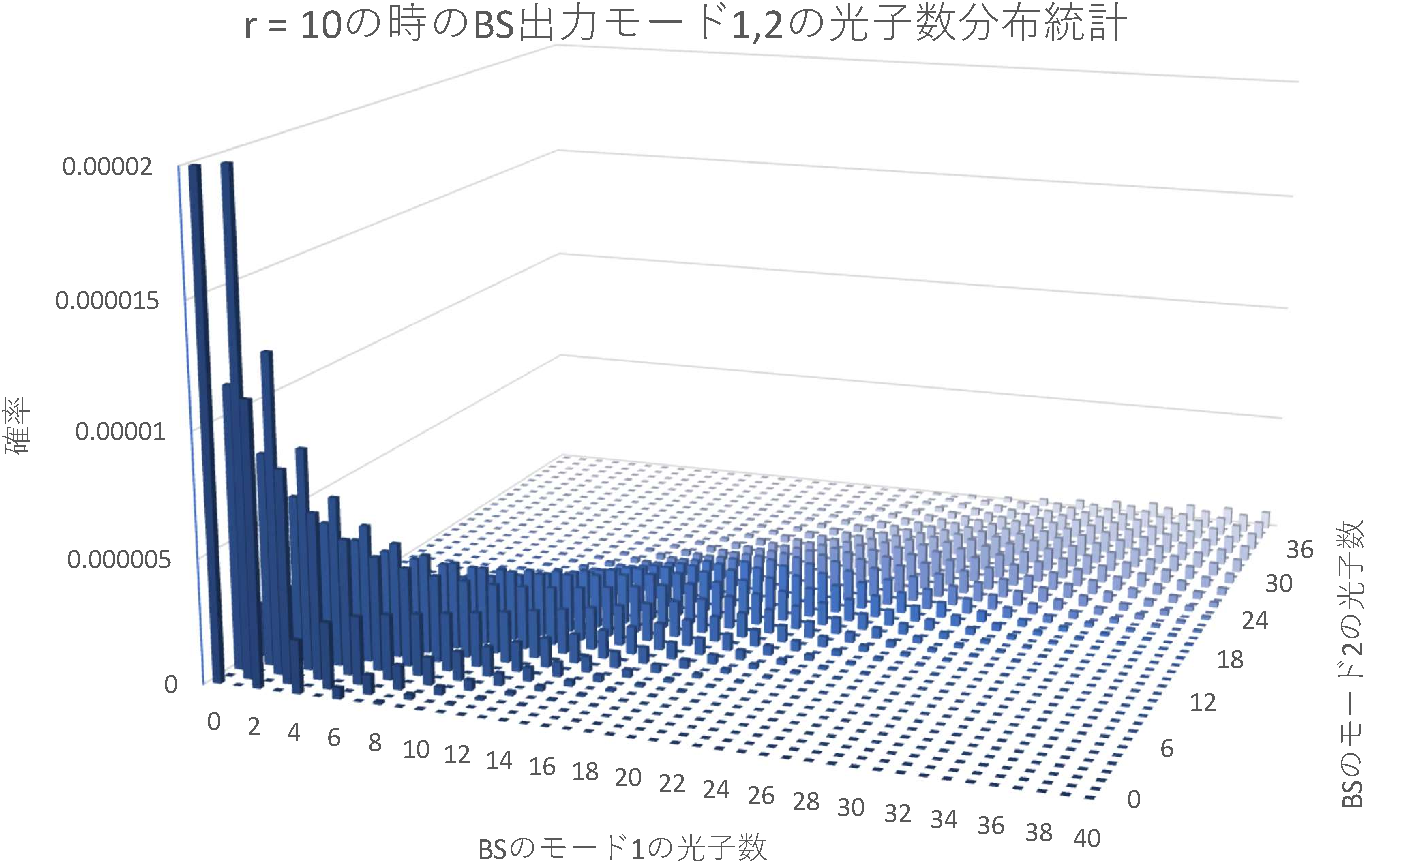
\includegraphics[width=0.9\linewidth]{./graphics/photon_sq.pdf}


\begin{itembox}[l]{問題}
	\vspace*{-0mm}
	\centering
	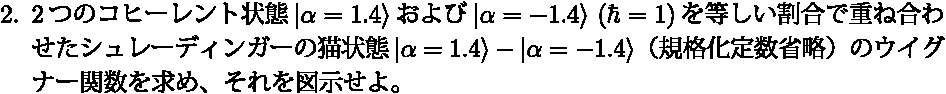
\includegraphics[width=1\linewidth]{./graphics/2.pdf}
\end{itembox}

最初にウィグナー関数と直行位相振幅を定義しておく。
\begin{gather*}
	W(x,p) = \frac{1}{2\pi \hbar} \int^{\infty}_{-\infty} \dd \xi \exp(-\frac{i}{\hbar}p\xi) \bra{x+ \frac{1}{2}\xi} \hat{\rho} \ket{x - \frac{1}{2}\xi}\\
	\hat{a} = \frac{\hat{x} + i \hat{p}}{\sqrt{2\hbar}}  , \qquad [\hat{x}, \hat{p}] = i\hbar
\end{gather*}
とりあえず猫状態を作るための変位演算子を$\hat{x},\hat{p}$で表すことから始めよう。以下$\hbar = 1$とする。
\begin{gather*}
	\alpha = \frac{x_0 + ip_0}{\sqrt{2}} ,\qquad x_0, p_0 \in \mathbb{R} \\
	D(\alpha) = e^{\alpha \hat{a}^\dagger - \alpha^* \hat{a}} = e^{i p_0 \hat{x} - i x_0 \hat{p}}
\end{gather*}
$\qty[\hat{A},[\hat{A},\hat{B}]]= \qty[\hat{B},[\hat{A},\hat{B}]]=0$のとき、Baker-Campbell-Hausdorffの公式より次が成り立つ。
\begin{gather*}
	e^{\hat{A} + \hat{B}}	=	e^{\hat{A}} e^{\hat{B}} e^{-\frac{1}{2}[\hat{A}, \hat{B}]}\\
	D(\alpha) = e^{ip_0 \hat{x}} e^{-ix_0 \hat{p}} e^{-\frac{1}{2} i x_0 p_0}
\end{gather*}
これを用いて猫状態が次のように表せる。なお適切に規格化してある。
\begin{gather*}
	\ket{\text{cat}} = \frac{1}{\sqrt{2(1-e^{-2|\alpha|^2})}} \qty(\ket{\alpha} - \ket{-\alpha} ) =\frac{1}{\sqrt{2(1-e^{-2|\alpha|^2})}}  \qty( D(\alpha) - D^\dagger(\alpha) )\ket{0}
\end{gather*}
$\hat{\rho} = \ket{\text{cat}} \bra{\text{cat}}$なので、
適当な$\ket{x}$の波動関数$\braket{x}{\text{cat}}$を求めたい。\\
一見複雑だが、$\braket{x}{0} = \psi_0 (x)$の組み合わせに帰結できる。
\begin{gather*}
	\braket{x}{\text{cat}} \propto \bra{x} \qty( D(\alpha) - D^\dagger(\alpha) ) \ket{0}\\
	D(\alpha) \ket{x}= e^{\frac{1}{2}i x_0 p_0} e^{ip_0 x} \ket{x + x_0}\\
	D^\dagger(\alpha) \ket{x} = e^{\frac{1}{2} i x_0 p_0} e^{-i p_0 x} \ket{x - x_0}\\
	\bra{x} D(\alpha) \ket{0} = e^{-\frac{1}{2} i x_0 p_0} e^{ip_0 x} \braket{x-x_0}{0}\\
	\bra{x} D^\dagger(\alpha) \ket{0} = e^{-\frac{1}{2} i x_0 p_0} e^{-ip_0 x} \braket{x+x_0}{0}
\end{gather*}
とりあえず真空場の波動関数を求めよう。\\
ヌリファイヤーは具体的な関数を解くために役立つ。
\begin{gather*}
	\bra{x} \hat{a} \ket{0} = \bra{x} \frac{\hat{x} + i \hat{p}}{\sqrt{2}}  \ket{0} = 0\\
	\bra{x} \hat{x} \ket{0} + i \bra{x} \hat{p} \ket{0} = x \psi_0(x) + i \qty( -i \frac{\dd}{\dd x} ) \psi_0 = 0\\
	\text{よって適当に解いて規格化すると} \qquad \psi_0 (x) = \qty( \frac{1}{\pi} )^{\frac{1}{4}} e^{- \frac{x^2}{2}}
\end{gather*}
よってこれを利用してウィグナー関数は次のようになる。
\begin{gather*}
	W(x,p) = \frac{1}{2\pi} \int^{\infty}_{-\infty} \dd \xi e^{-i p \xi} \braket{x+\frac{1}{2} \xi}{\text{cat}} \braket{\text{cat}}{x - \frac{1}{2} \xi}\\
	= \frac{1}{2\pi} \int^{\infty}_{-\infty} \dd \xi e^{-i p \xi} \frac{1}{2(1-e^{-2|\alpha|^2})} \qty{ \mel{x + \frac{\xi}{2}} {D(\alpha)}{0} - \mel{x + \frac{\xi}{2}} {D^\dagger(\alpha)}{0}}\\
	\times \qty{ \mel{0} {D^\dagger(\alpha)}{x - \frac{\xi}{2}} - \mel{0} {D(\alpha)}{x - \frac{\xi}{2}} }\\
	= \frac{1}{2\pi (1-e^{-2|\alpha|^2})} \qty( e^{-(x-x_0)^2 - (p- p_0)^2} + e^{-(x+x_0)^2 - (p+p_0)^2} - 2e^{-x^2 - p^2} \cos{2(x_0 p - x p_0)})
\end{gather*}
これを3Dプロットすると次のようになる。ただし$\alpha=1.4$\\
$x=0,y=0$でウィグナー関数のネガティビティーが見られるため、非古典状態なことが伺える。\\
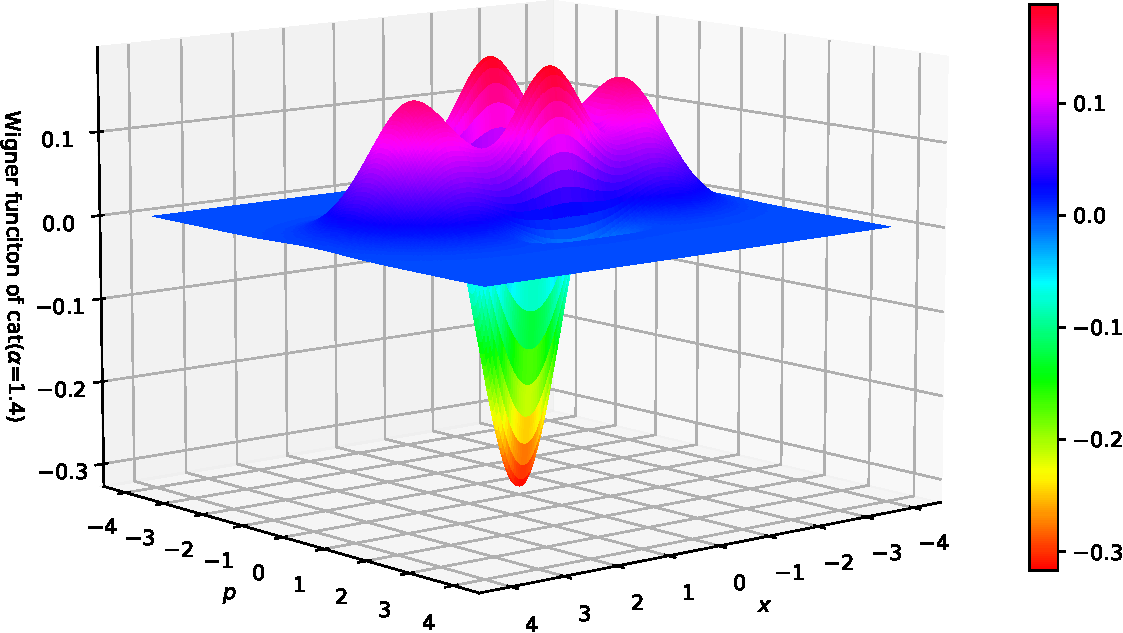
\includegraphics[width=0.9\linewidth]{./graphics/wigner.pdf}


\begin{itembox}[l]{問題}
	\vspace*{-0mm}
	\centering
	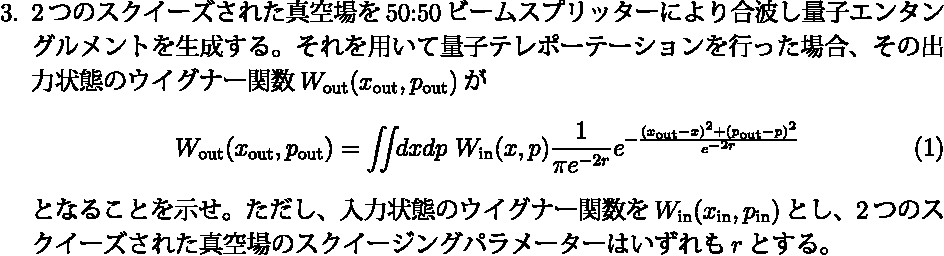
\includegraphics[width=1\linewidth]{./graphics/3.pdf}
\end{itembox}

検討するビームスプリッターネットワークは図のものとする。\\
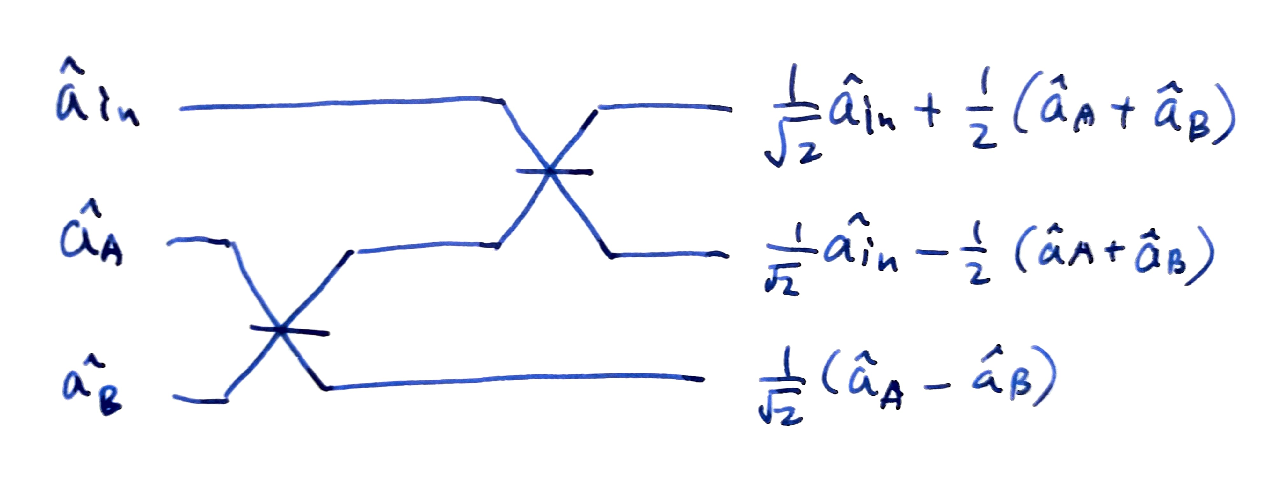
\includegraphics[width=1\linewidth]{./graphics/BSnet.pdf}
とりあえずスクイージング状態のウィグナー関数を書き下したい。\\
A,Bの2モードの真空場のウィグナー関数は次のようになる。
\begin{gather*}
	W_0(x_A,p_A)W_0(x_B,p_B)
	=
	\frac{1}{\sqrt{\pi}}
	e^{-x_A^2-p_A^2}
	\frac{1}{\sqrt{\pi}}
	e^{-x_B^2-p_B^2}
\end{gather*}
Aをpスクイーズ、Bをxスクイーズとする。
\begin{gather*}
	W_\mr{a-sq}(x_A,p_A)
	W_\mr{sq}(x_B,p_B)
	=
	W_0(e^{-r} x_A,e^r p_A)W_0(e^r x_B,e^{-r} p_B)\\
	= \frac{1}{\pi} e^{ -e^{-2r}(x_A^2 + p_B^2) - e^{2r}(x_B^2 + p_A^2)}
\end{gather*}
$\hat{a}_\mr{in}$モードのウィグナー関数を$W_\mr{in}(x_\mr{in},p_\mr{in})$とする。\\
ビームスプリッターネットワークの出力のウィグナー関数は次のようになる。
\begin{gather*}
	W_\mr{en} \qty(
		\begin{alignedat}{2}
			&\frac{1}{\sqrt{2}} x_\mr{in} + \frac{1}{2}(x_A+x_B)&	&,\frac{1}{\sqrt{2}} p_\mr{in} + \frac{1}{2}(p_A+p_B);\\
			&\frac{1}{\sqrt{2}} x_\mr{in} - \frac{1}{2}(x_A+x_B)&	&,\frac{1}{\sqrt{2}} p_\mr{in} - \frac{1}{2}(p_A+p_B);\\
			&\frac{1}{\sqrt{2}} (x_A - x_B)						&	&,\frac{1}{\sqrt{2}} (p_A - p_B)
		\end{alignedat}
	)
	=
	W_\mr{in}(x_\mr{in},p_\mr{in})
	W_\mr{a-sq}(x_A,p_A)
	W_\mr{sq}(x_B,p_B)
\end{gather*}
適当に変数変換して出力を上から連番で振り分けると次のようになる。
\begin{align*}
	W_\mr{en}(x_1,p_1;x_2,p_2;x_3,p_3)
	=&
	W_\mr{in} \qty( \frac{1}{\sqrt{2}} (x_1+x_2), \frac{1}{\sqrt{2}} (p_1+p_2) )\\
	& \times W_\mr{a-sq} \qty( \frac{1}{2} (x_1-x_2) + \frac{1}{\sqrt{2}} x_3, \frac{1}{2} (p_1-p_2) + \frac{1}{\sqrt{2}} p_3)\\
	& \times W_\mr{sq} \qty( \frac{1}{2} (x_1-x_2) - \frac{1}{\sqrt{2}} x_3, \frac{1}{2} (p_1-p_2) - \frac{1}{\sqrt{2}} p_3 )
\end{align*}
その後適当にベル測定を行い、フィードフォワードして量子テレポーテーションとなる。\\
図のように測定するとする。\\
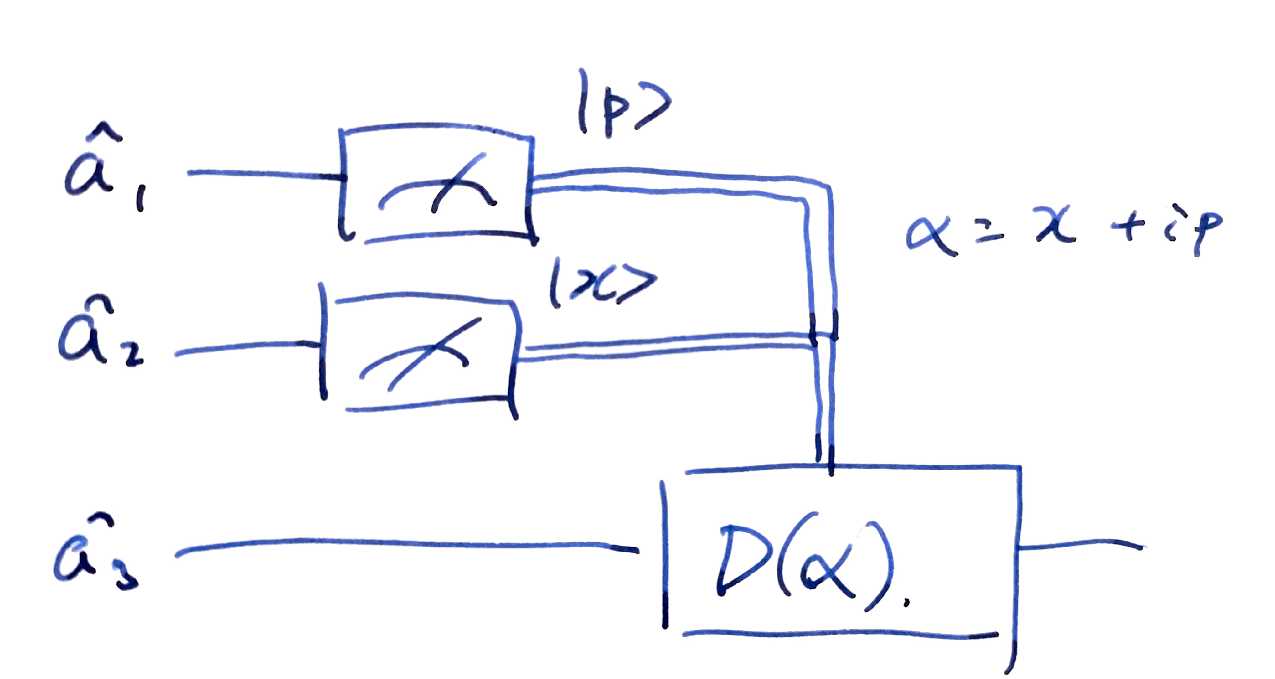
\includegraphics[width=0.5\linewidth]{./graphics/disp.pdf}\\
ベル測定によって$x,p$の結果が得られたら、x方向に$\sqrt{2}x$、y方向に$\sqrt{2}p$ディスプレイスメントする。
\begin{gather*}
	\alpha = \frac{\sqrt{2}x + i \sqrt{2}p}{\sqrt{2}} = x + ip
\end{gather*}
出力されるウィグナー関数は荒削りに書くとこうなる。まだ雰囲気は掴めない。\\
\begin{gather*}
	W_\mr{out}(x_\mr{out}, p_\mr{out}) = \iint \dd x_1 \dd p_1 \dd x_2 \dd p_2 W_\mr{en} (x_1,p_1;x_2,p_2;x_\mr{out} - \sqrt{2}x_2,p_\mr{out} - \sqrt{2}p_1)
\end{gather*}
これを適当に変数変換して、もっとわかりやすい形に書き直そう。\\
次のような変数に置き換える。
\begin{gather*}
	x = \frac{1}{\sqrt{2}}( x_1 + x_2 ), \quad p = \frac{1}{\sqrt{2}} ( p_1 + p_2 )\\
	x' =  \frac{1}{\sqrt{2}}( x_1 - x_2 ), \quad p' = \frac{1}{\sqrt{2}} ( p_1 - p_2 )
\end{gather*}
したがって変形を繰り返していくことで、\\
量子テレポーテーションされたウィグナー関数は畳み込みで表せるようになった。\\
しかしながら、問題で示す式とは異なり$e^{-2r} \rightarrow 2e^{-2r}$となった。\\
どうしてだろうか?
\begin{gather*}
	W_\mr{out}(x_\mr{out}, p_\mr{out}) =\\
	\iint \dd x \dd p \dd x' \dd p'
	W_\mr{in} (x,p) 
	W_\mr{a-sq} \qty( \frac{1}{\sqrt{2}} ( x_\mr{out} + 2x' - x ), \frac{1}{\sqrt{2}} (p_\mr{out} - p))
	W_\mr{sq} \qty(  \frac{1}{\sqrt{2}} (-x_\mr{out} + x)   ,   \frac{1}{\sqrt{2}} ( -p_\mr{out} + 2p' + p ) )\\
	= \iint \dd x \dd p \dd x' \dd p' W_\mr{in} (x,p) \frac{1}{\pi} e^{- \frac{(p_\mr{out} - p)^2 + (x_\mr{out} - x)^2}{2 e^{-2r}}}
	e^{-\frac{(x_\mr{out}+2x' - x)^2 + (p_\mr{out} - 2p' -p)}{2e^{2r}}}\\
	= \iint \dd x \dd p W_\mr{in}(x,p) \frac{1}{2\pi e^{-2r}} e^{- \frac{(p_\mr{out} - p)^2 + (x_\mr{out} - x)^2}{2 e^{-2r}}}
\end{gather*}

\begin{itembox}[l]{問題}
	\vspace*{-0mm}
	\centering
	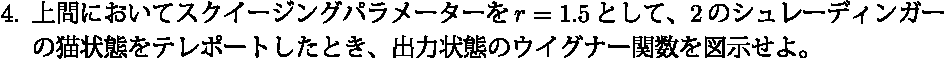
\includegraphics[width=1\linewidth]{./graphics/4.pdf}
\end{itembox}

次が正しいとする。
\begin{gather*}
	W_\mr{out}(x_\mr{out}, p_\mr{out}) = \iint \dd x \dd p W_\mr{in}(x,p) \frac{1}{\pi e^{-2r}} e^{- \frac{(p_\mr{out} - p)^2 + (x_\mr{out} - x)^2}{ e^{-2r}}}
\end{gather*}










\bibliography{
  citation.bib
}
\bibliographystyle{junsrt}

\end{document}
